\documentclass{report}
\usepackage{graphicx}
\usepackage{subfigure}
\usepackage{parskip}
\usepackage{algorithm}
\usepackage{algorithmicx}
\usepackage{algpseudocode}
\usepackage{amsmath}
\usepackage{float}


\floatname{algorithm}{Algorithm}
\renewcommand{\algorithmicrequire}{\textbf{Input:}}
\renewcommand{\algorithmicensure}{\textbf{Output:}}


\begin{document}

\title{SOEN 6011: SOFTWARE ENGINEERING PROCESSES\\ Gamma Function Scientific Calculator}
\author{Github: https://github.com/aishangchixiang/SOEN6011\\Wenshu Li 40203982}
\maketitle






% This will generate a table of contents
\tableofcontents
\newpage
\section{Introduction}
\subsection{Discription}
In mathematics, the gamma function is one commonly used extension of the factorial function to complex numbers\cite{enwiki:1102404428}, is a meromorphic function defined in the complex range, usually written so that negative integers and 0 are its first order poles.There are various definitions of the gamma function, we selected three of them here:
\begin{itemize}
\item For any positive integer n,
\\$$\Gamma \left ( n\right ) = \left ( n-1 \right )!$$
\item Derived by Daniel Bernoulli, for complex numbers with a positive real part, the gamma function is defined via a convergent improper integral:
\\$$\Gamma \left ( z\right ) = \int_{0}^{+\infty} x^{z-1} e^{-x}\mathrm{d}x,  \Re\left ( z \right )>0$$
\item The gamma function on real number field is defined as:
\\$$\Gamma \left ( x \right ) =\int_{0}^{+\infty } t^{x-1} e^{-t} \mathrm{d}t \left (  x>0\right ) $$
\end{itemize} 

\begin{figure}[h]
\caption{Gamma function}
\centering
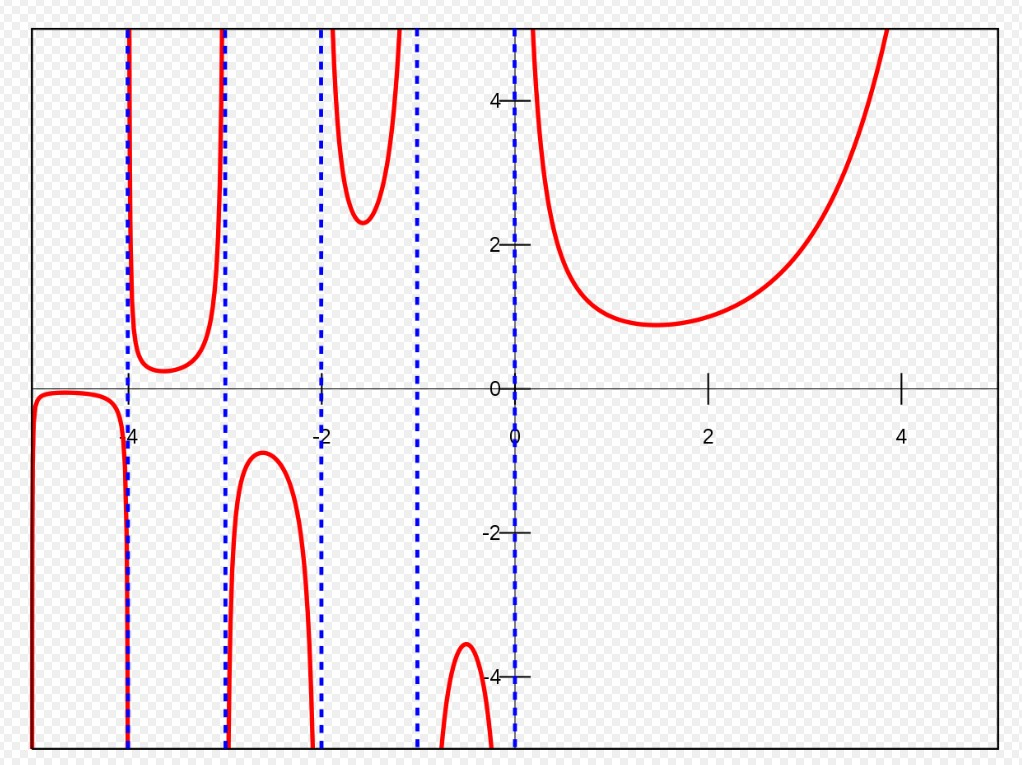
\includegraphics[width=0.5\textwidth]{gamma}
\end{figure}
 

\subsection{Domain}
All complex numbers except those whose real part are non-positive integers.
\\$$C/\{n\in Z, n\le 0\}$$
\subsection{Co-Domain}
All real numbers excluding zero.
\\$$\left ( -\infty,0  \right )\cup \left ( 0,+\infty  \right )$$
\subsection{Properties}
%https://en.wikipedia.org/wiki/Gamma_function#Properties
One of the important functional equatuations for the gamma fucntion is Euler's reflection formula:
\\$$\Gamma \left ( 1-z \right ) \Gamma \left ( z \right ) =\frac{\pi }{\sin \pi z},  z \notin Z $$ 
\subsection{Perticular Values}
%https://en.wikipedia.org/wiki/Gamma_function#Particular_values
It is easy to find some special values for the gamma function on the web, which can be used as subsequent test cases. Including up to the first 20 digits after the decimal point, some of particular values of the gamma function are\cite{enwiki:1102366902}:
\begin{itemize}
\item $\Gamma \left ( \frac{1}{2}  \right ) =\sqrt{\pi }  \approx +1.77245385090551602729$
\item $\Gamma \left ( 1  \right ) =0! = +1$
\item $\Gamma \left ( \frac{3}{2}  \right ) =\frac{\pi }{2}   \approx +0.88622692545275801364$
\item $\Gamma \left ( 2 \right ) =1!=+1$
\item $\Gamma \left ( \frac{5}{2}  \right ) =\frac{3\sqrt{\pi } }{4} \approx +1.32934038817913702047$
\item $\Gamma \left ( 3  \right ) =2! \approx +2$
\item $\Gamma \left ( \frac{7}{2}   \right ) =\frac{15\sqrt{\pi } }{8}  \approx +3.32335097044784255118$
\item $\Gamma \left ( 4 \right ) =3!=+6$
\end{itemize}

\subsection{Stakeholders and Context of Use Model}
\begin{itemize}
\item User1: Mathematicians and researchers in the fields of calculus, mathematical analysis, statistics.
\item User2: Algorithm designers, researchers,engineers in the field of scientific computing in computer and software engineering.
\item User3: People with low maths and programming background who need to obtain the values of gamma function.
\end{itemize}
As can be seen from Figure 2, the user can input the data he wants to input through the interactive system, such as the value of some independent variables, and then the data is converted into data that can be used by the core algorithm part, and the result is calculated and then presented to the user through the interactive system, which includes error handling, such as the user inputting illegal characters that can cause the calculator not to recognize, etc.
\begin{figure}[h]
\caption{Context of use model}
\centering
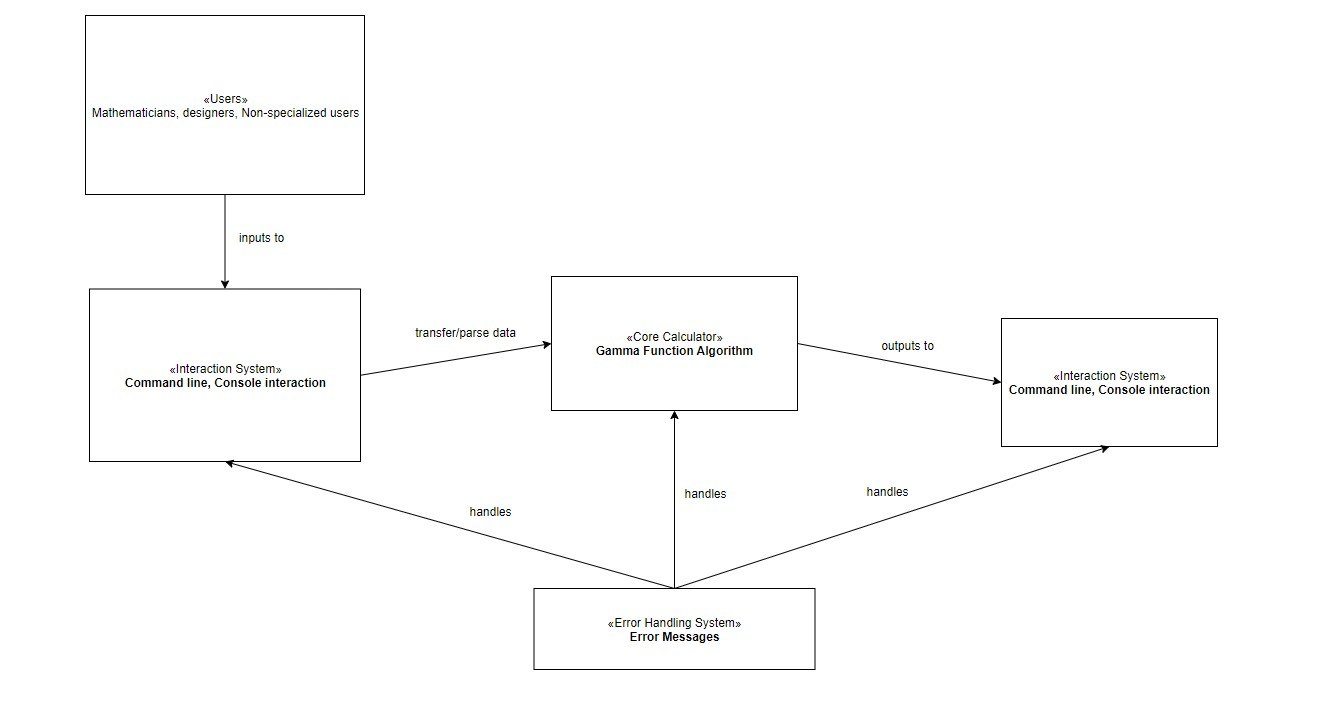
\includegraphics[width=0.95\textwidth]{context of use}
\end{figure}



\section{Requirements}
\subsection{Assumptions}
\begin{itemize}
\item A1: We shall only consider the positive value as input value, 
\item A2: We shall only consider the real number as input value, ignore the imaginary part.
\item A3: We can accept a certain error in the calculation results, but it needs to be within a certain range.
\item A4: The error of the calculation result should be within a certain range.
\end{itemize}

\subsection{Functional Requirements}
\begin{itemize}
\item FR1-A3: When the user enters a value that is a non-numeric character, we will give the prompt "Error!". 
\item FR2-A1: When the user enters a negative value, the function will return "Negative input is not allowed.".
\item FR3-A1: When the function value exceeds the maximum the value of a double type variable or equals to zero, the function will return "Infinity".
\item FR4-A4: When the input value is a positive integer, the error between the output value and the real value shall be less than 0.001, individual errors greater than 0.001 are allowed, but must be less than 0.1.
\end{itemize}

\subsection{Non-functional Requirements}
\begin{itemize}
\item NFR1: The calculator project shall be maintainable, the code is saved by the github repository, and all functions in the program can be modified and maintained.
\item NFR2: The calculator project shall be portable, the project can be run on a computer with a java environment and does not require high computer hardware and computing power.
\item NFR3: The calculator project shall be usable, it can be used by different users to calculate the value of the gamma function.
\end{itemize}

\section{Algorithm}
\subsection{Integrals Method}
\subsubsection{Description}
The first algorithm is based on the Gamma function formula derived by Daniel Bernoulli, using an approximating integrals method called trapezoidal rule\cite{enwiki:1095730995}. It is used for initial value problems. In calculus, the trapezoidal rule is a technique for approximation the definite integral. This algorithm involves two sub-functions. One is the power function, which given base and exponent as double type arguments, returns $base^{exponent}$. And the exp function, which given exponent as double type argument, returns $e^{exponent}$ .

\subsection{Lanczos Approximation}
\subsubsection{Description}
The second algorithm is based on Lanczos approximation\cite{enwiki:1095709670}. In mathematics, the Lanczos approximation is a method for computing the gamma function numerically, published by Cornelius Lanczos in 1964. It is a practical alternative to the more popular Stirling's approximation\cite{enwiki:1068285162} for calculating the gamma function with fixed precision. This algorithm also involves power function, exp function, and sqrt function which given one double type argument, returns square root.
\subsection{Pseudocode} 
Pseudocode generally does not actually obey the syntax rules of any particular language; there is no systematic standard form\cite{enwiki:1101060705}. So, according to the rules of java programming language and the basic specification of pseudo-code, the following pseudo-code is written, which contains the code of Algorithm 1 and Algorithm 2, which involves some sub-functions such as pow(), sin(), ln(), etc. The principle of their implementation is to replace the original expression with a level form represented only by addition, subtraction, multiplication and division, according to the Taylor series\cite{enwiki:1097849466}, which is implemented by a loop or recursive method. The formula is as follows:
\begin{itemize}
\item The power function:
\\ $$pow(a,x)=a^{x} = e^{x\ln{a} }=1+\frac{x\ln{a}}{1!}+\frac{(x\ln{a})^{2}}{2!}+\frac{(x\ln{a})^{3}}{3!}+\cdots \ (-\infty < x < \infty)$$
\item The logarithm function:
\\ $$\ln(x)=\ln{(\frac{1+y}{1-y})}=2(\frac{1}{1}+\frac{1}{3}y^2+\frac{1}{5}y^4+\frac{1}{7}y^6+\frac{1}{9}y^8+\cdots )  \ (-\infty < x < \infty)$$
\item The sin function:
\\ $$sin(x)= x-\frac{x^{3} }{3!} +\frac{x^{5}}{5!}-\cdots \ (-\infty < x < \infty)$$
\end{itemize}

\begin{algorithm}
	\caption{Calculate Gamma function using integrals method} 
	\begin{algorithmic}[1]
	\begin{footnotesize}
		\Require Input value of x
		\Ensure Output value of Gamma function
		\Function{$f_y$}{$x$}
			\State \Return {$s^{x-1}*e^{-s}$}
		\EndFunction
		\State
		\Function{$gamma$}{$x$}
			\State $output \gets Error$
			\If{$x<0$}
				\State $result \gets Negative \ input \ is \ not \ allowed.$
			\ElsIf{$x>110$}
				\State $result \gets Infinity$
			\Else
			\State $result \gets 0, intervalGap \gets 10^{-3},i \gets 0$
			\While{$i<a \ particular \ value$}
				\State $result \gets result + \frac{1}{2}*intervalGap*\left ( f_y\left ( i \right ) +y\left (  i-intervalGap\right )  \right )$
				\State $i \gets i+intervalGap$
			\EndWhile
			\State $output \gets result$
			\EndIf
			\State \Return {$output$}
		\EndFunction
		\State
		\Function{$pow$}{$base, power$}
		\State $temPower \gets power * logarithm(base)$
		\State $sum \gets 1.0, flag \gets 0$
		\If{$tempPower < 0$}
			\State $tempPower \gets temPower * -1$
			\State $flag \gets 1$
		\EndIf
		\State $ratio \gets tempPower$
		\For{$i\ in\ \left(2,500\right)$}
			\State $ratio \gets ratio * temPower / i$
			\State $sum \gets sum + ratio$
		\EndFor
		\If{$flag == 1$}
			\State $sum \gets 1.0 / sum$
		\EndIf
		\State \Return $sum$
		\EndFunction
		\State
		\Function{$logarithmFunction$}{$base$}
			\State $sum \gets 0$
			\State $multiple \gets 1.0$
			\For {$ i\ in\ \left(1,10000\right)$}
				\State $multiple = multiple * ((base-1)/(base+1))$
				\If {$i\mod2!=0$}
					\State $sum = sum + multiple/i$
				\EndIf
			\EndFor
			\State \Return {$2*sum$}
		\EndFunction
	\end{footnotesize}
	\end{algorithmic}
\end{algorithm}
\begin{algorithm} 
	\caption{Calculate Gamma function using Lanczos approximation} 
	\begin{algorithmic}[1]
	\begin{footnotesize}
		\Require Array p as a coefficients, and a constant EPSILON
		\Ensure Output value of Gamma function
		\Function{$gamma$}{$x$}
		\If{$x<0$}
			\State \Return {$Negative \ input \ is \ not \ allowed.$}
		\EndIf
		\If{$x<0.5$}
			\State \Return {$ \frac{\pi}{\sin \left ( \pi*z  \right )*gamma\left ( 1-z \right ) } $}
		\Else
			\State $x \gets x-1$
			\State $z \gets 0.99999999999980993$
			\For{$\left (i,pval\right) in \ p$}
				\State $ z \gets z+\frac{pval}{x+i+1} $
			\EndFor
			\State $t \gets x+length \left (p \right)-0.5$
			\State $m \gets \sqrt{2*\pi }*pow\left ( t,\left ( x+0.5 \right )  \right ) *exp\left ( -t \right ) *z$
		\EndIf
		\State \Return $m$
		\EndFunction
		\State
		\Function{$sin$}{$x$}
			\State $sum \gets 0$
			\State $flag \gets 1$
			\For{$i\ in\ \left(1,500 \right)$}
				\If{$i\ mod\ 2 == 1$}
					\State $N \gets 0$
					\State $D \gets 0$
					\For{$j\ in\ \left(1,i \right)$}
						\State $N \gets N * x$
						\State $D \gets D * j$
					\EndFor
					\State $sum \gets sum + flag * \frac{N}{D}$
				\State $flag \gets flag * -1$
				\EndIf
			\EndFor	
		\EndFunction
	\end{footnotesize}
	\end{algorithmic}
\end{algorithm}
\clearpage
\subsection{Advantages and Disadvantages}
\subsubsection{Algorithm 1}
Advantages:
\begin{enumerate}
\item Using the the integral method makes the algorithm more intuitive and easy to understand.
\item More precise calculations results can be obtained.
\item The entire algorithm involves loops without recurtion, it requires less memory from computing devices.
\end{enumerate}
Disadvantages:
\begin{enumerate}
\item When the input value is large, it takes significantly longer to produce the result.
\end{enumerate}

\subsubsection{Algorithm 2}
Advantages:
\begin{enumerate}
\item The algorithm makes computing the gamma function becomes a matter of evaluating only a small number of elementary functons and multiplying by stored constants. Simpler to implement.
\item Calculation time is almost independent of the input value.
\end{enumerate}
Disadvantages:
\begin{enumerate}
\item Less precise calculations results than Algorithm 1.
\item The coefficients and Constants that we give in advance are not always precise and accurate.
\end{enumerate}

\subsection{Final Decision}
The algorithm 1 is chosen for implementation. Because it could provide more precise results, although it is theoretically slower than the second one, there is no much difference in terms of actual execution time. Figure 3 below shows the mind map.
\begin{figure}[H]
\centering
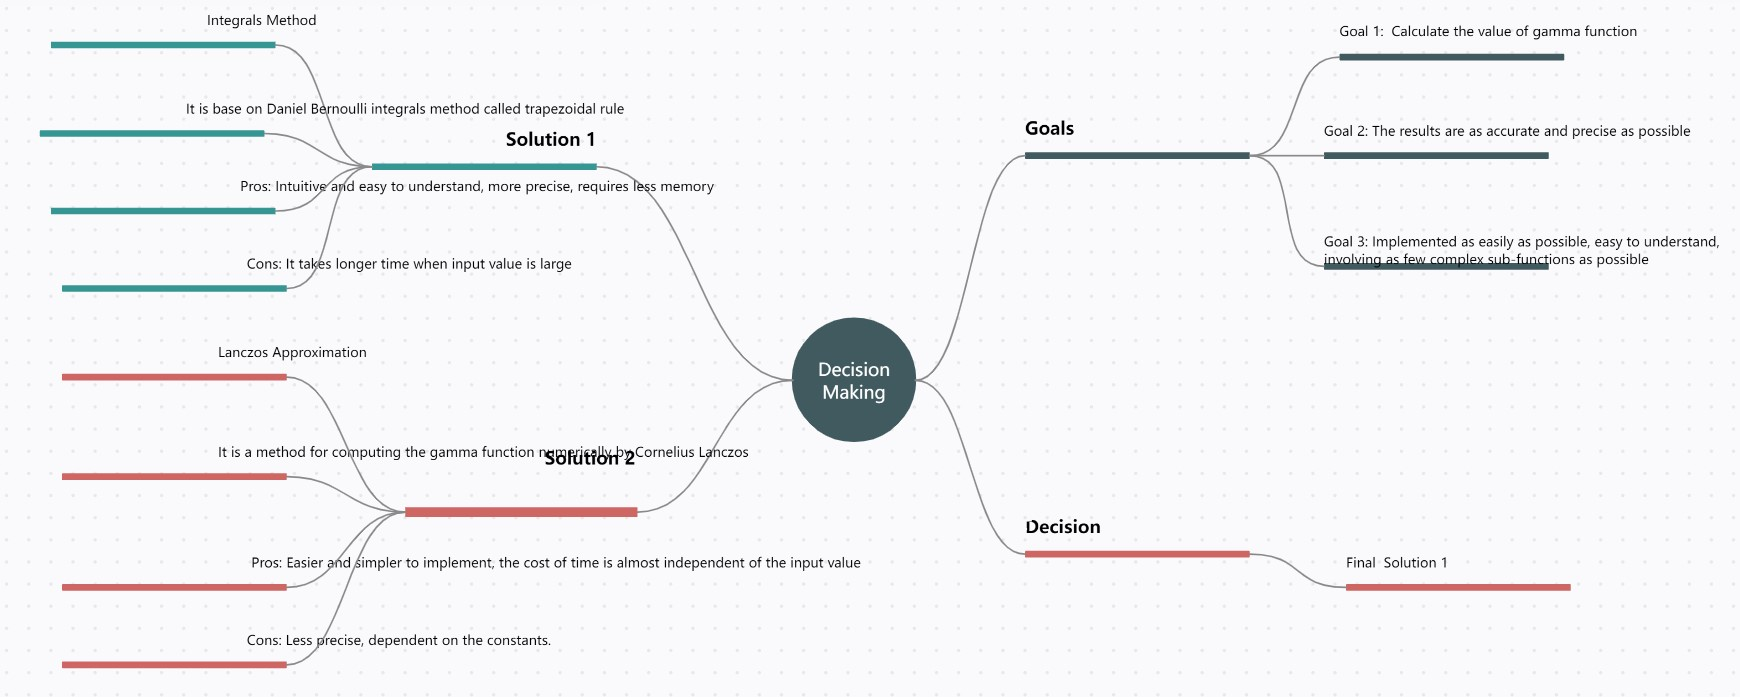
\includegraphics[width=0.60\textwidth]{mind map}
\caption{Mind map}
\end{figure}


\newpage
\section{Implementation}
\subsection{Evidence of Debugger}

\begin{figure}[H]
    \centering
    \subfigure[debug\_1]{
        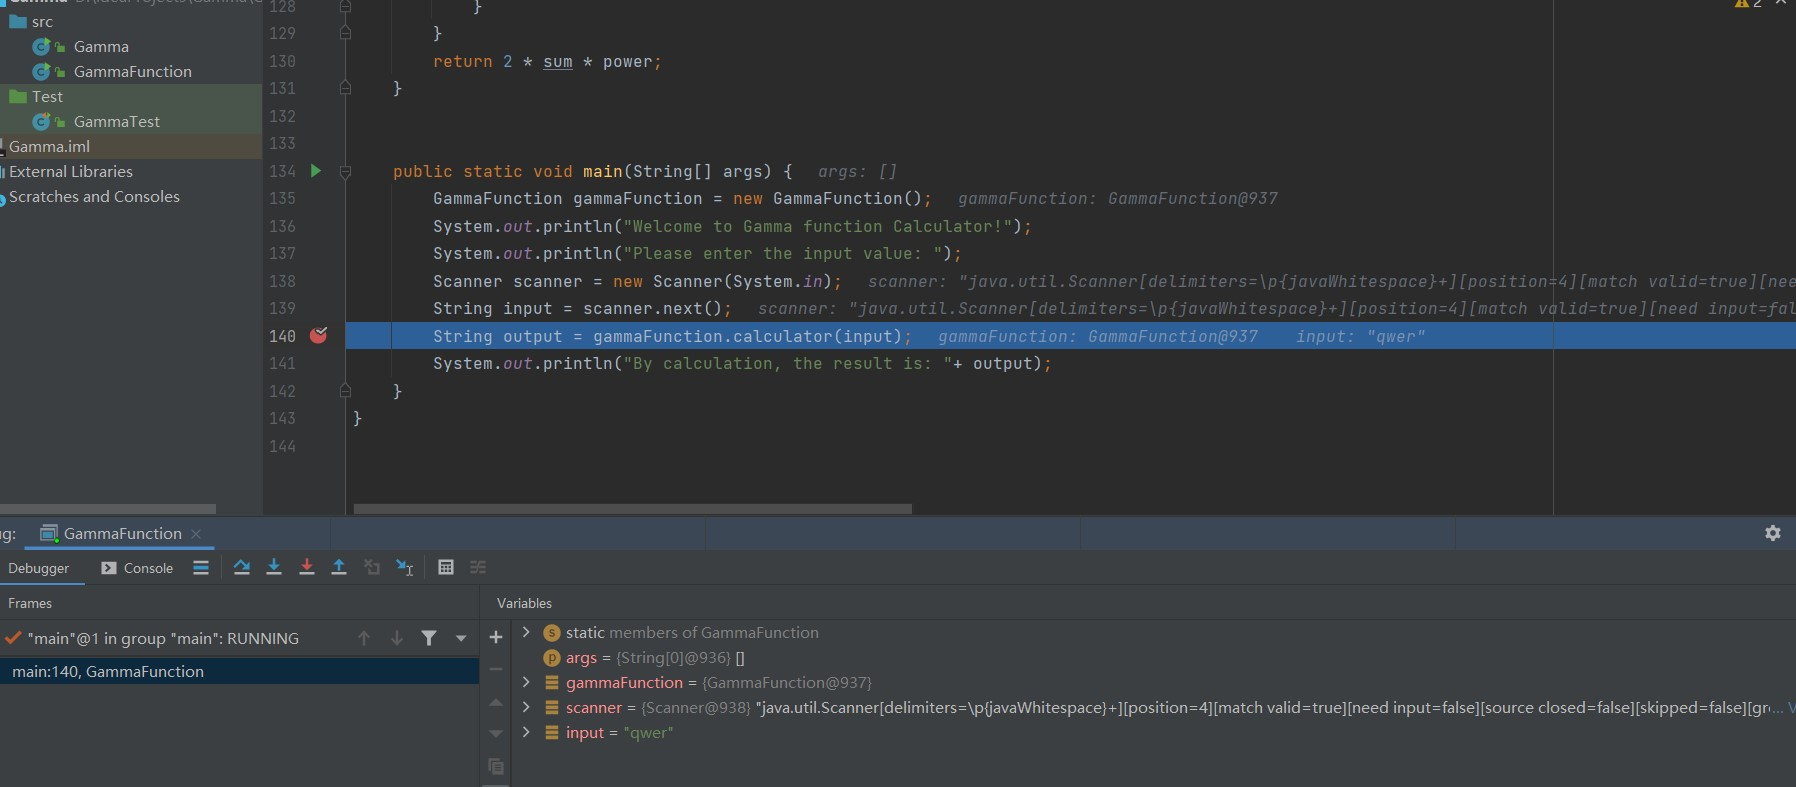
\includegraphics[width=5.5cm]{debug_1}
    }
    \subfigure[debug\_2]{
	 		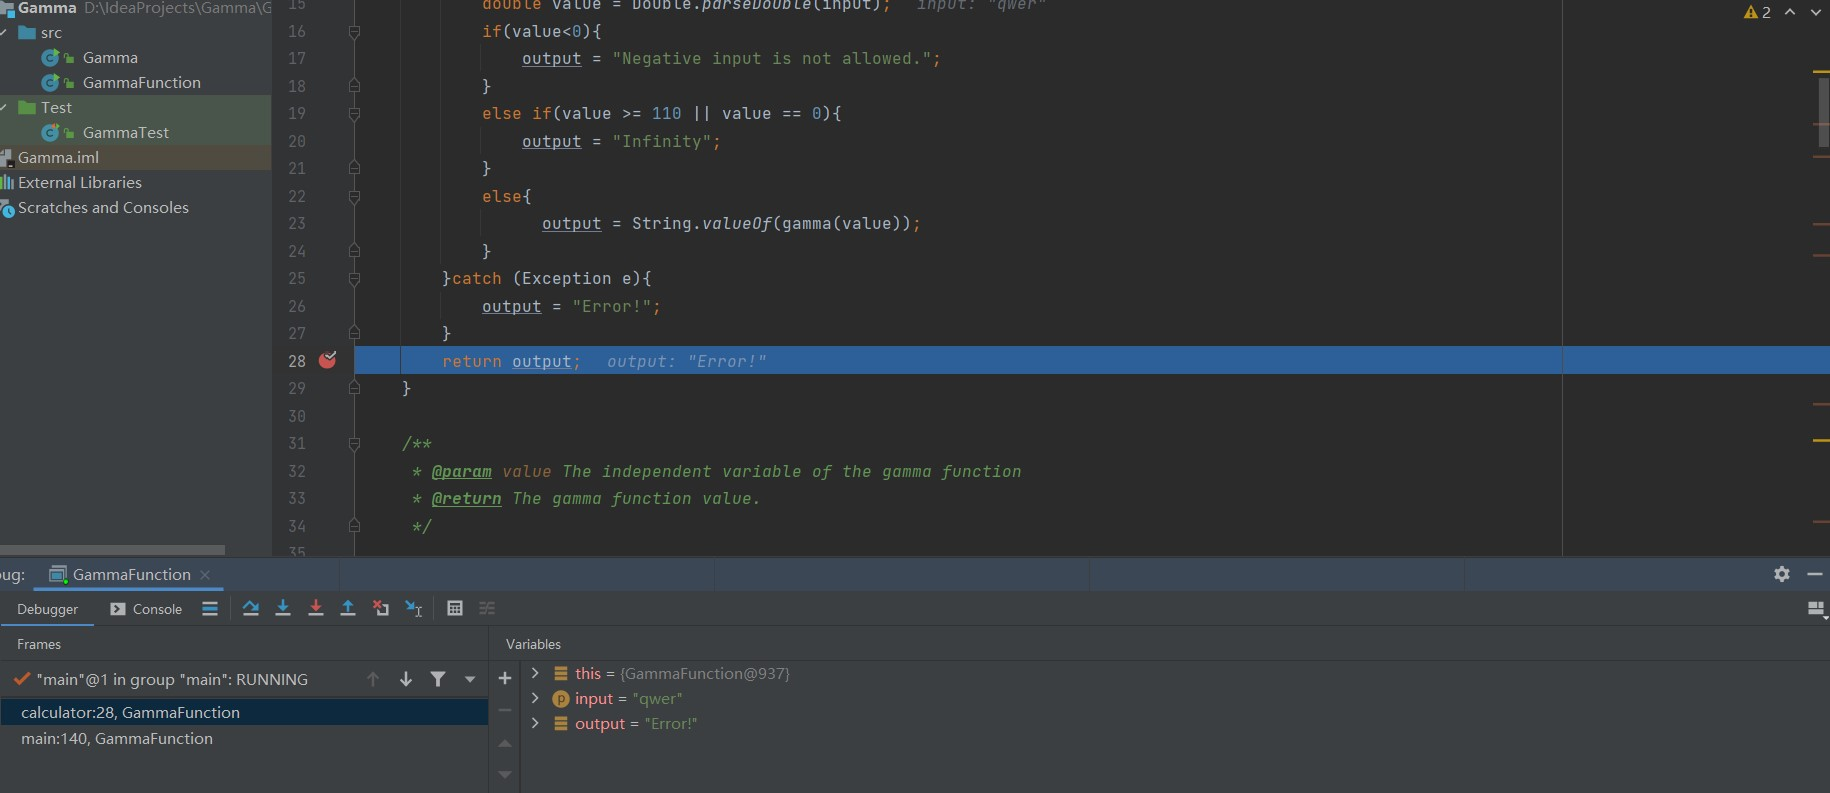
\includegraphics[width=5.5cm]{debug_2}
    }
    \quad    
    \subfigure[debug\_3]{
    		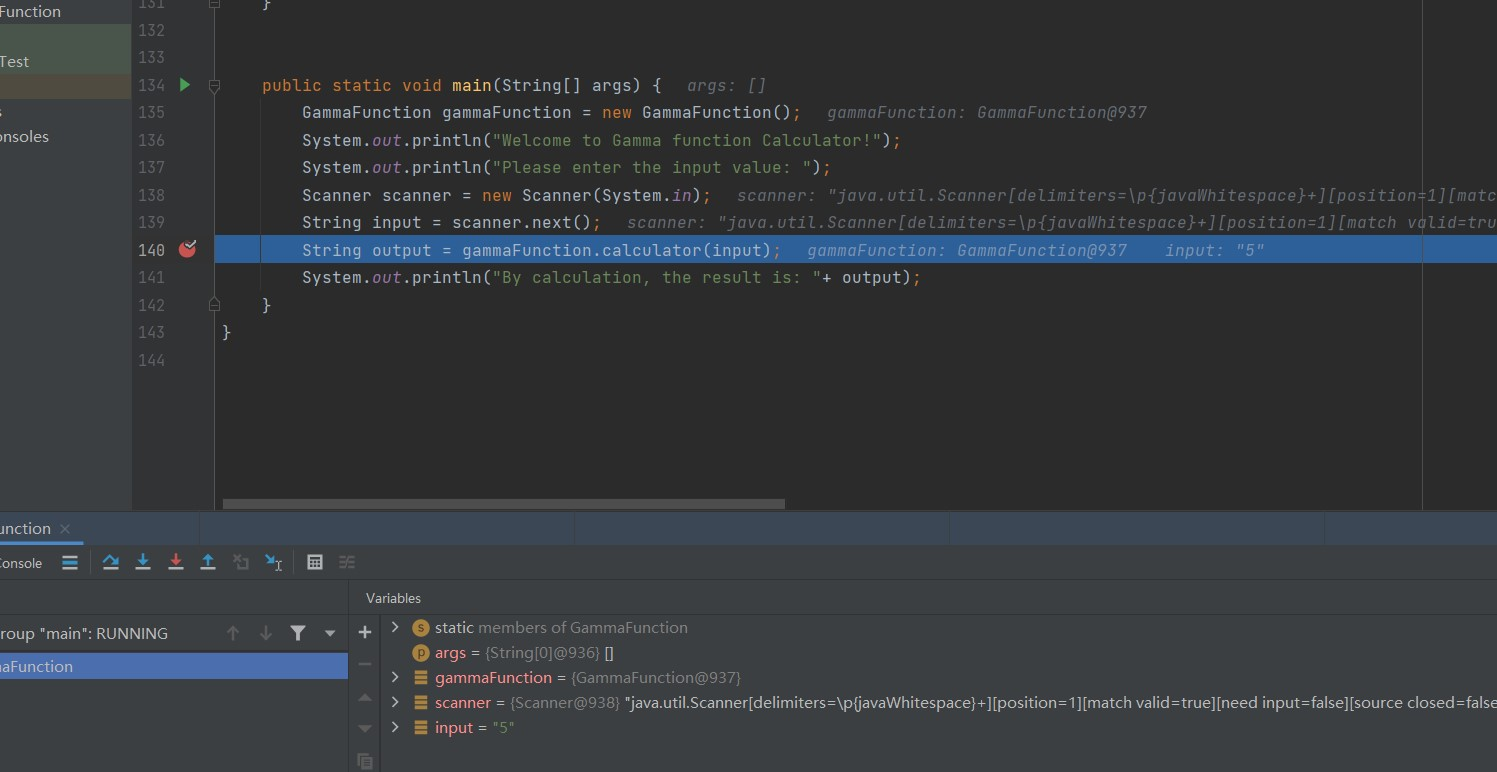
\includegraphics[width=5.5cm]{debug_3}
    }
    \subfigure[debug\_4]{
			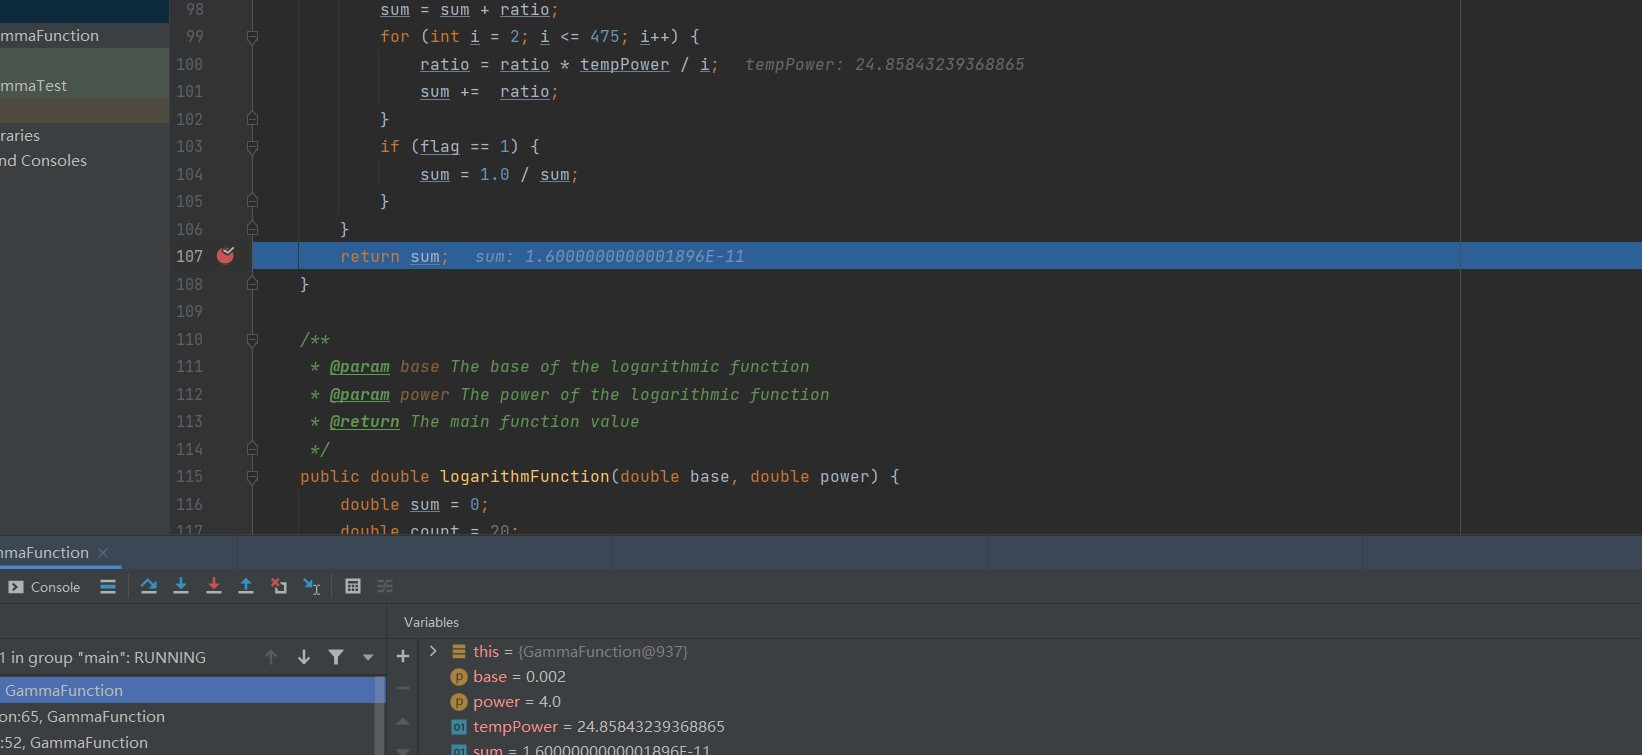
\includegraphics[width=5.5cm]{debug_4}
    }
    \caption{This is the Screenshot for debuggers}
\end{figure}

\subsection{Evidence of Use of Pragmatic Quality Checking Tool}
For Pragmatic Quality Checking, I used QAPLug, an IDE plugin that automatically evaluates code and projects in terms of performance, maintainability, executability, reliability, and usability, and the results are shown in the Figure 5 below.
\begin{figure}[htbp]
\centering
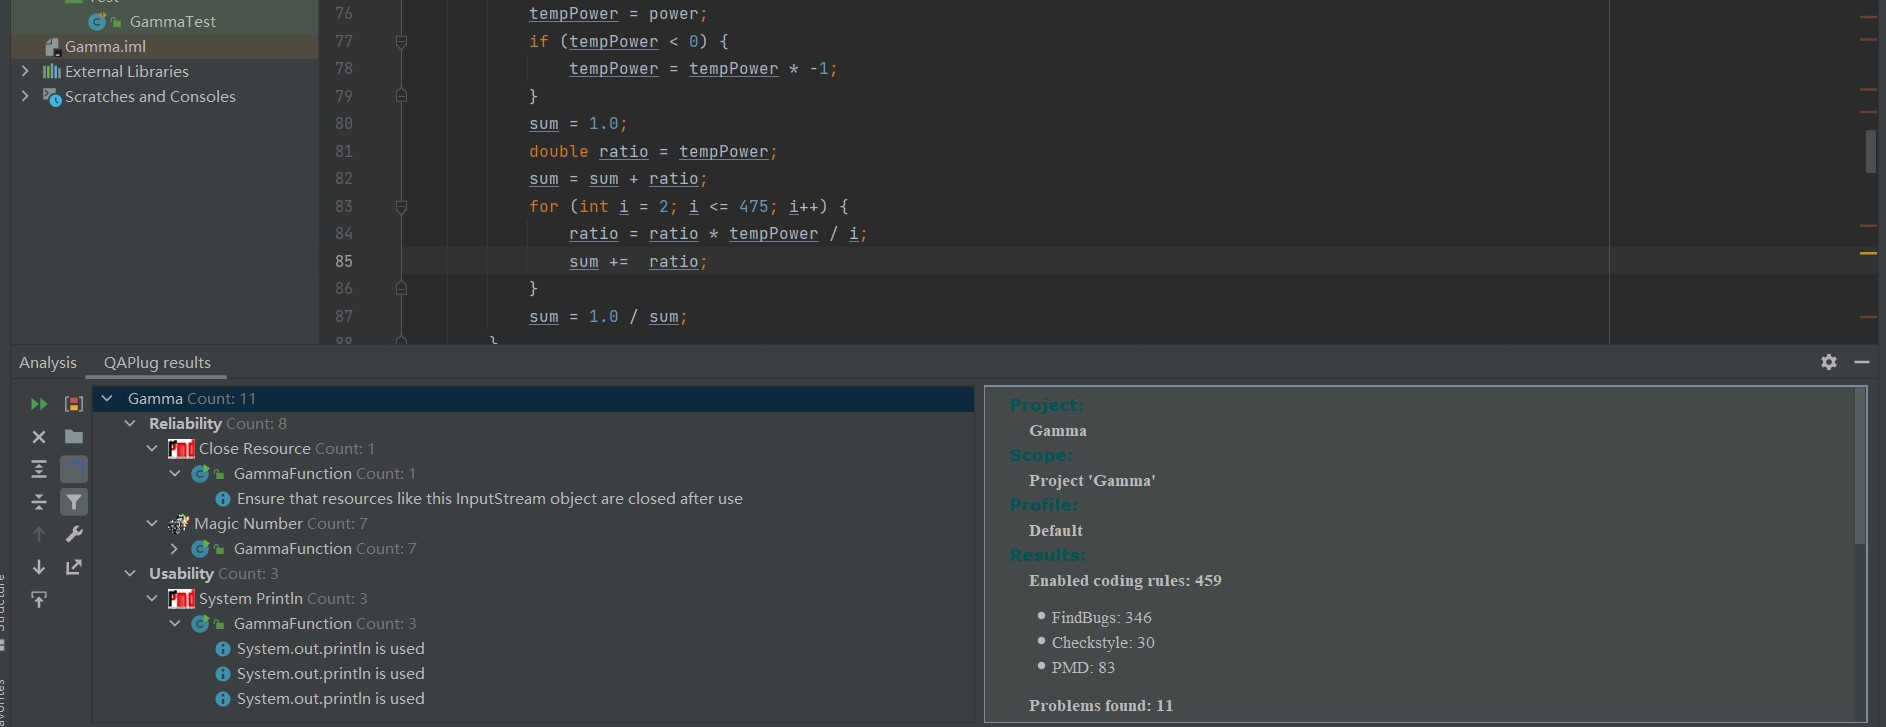
\includegraphics[width=0.75\textwidth]{QA_1}
\caption{QA}
\end{figure}

\newpage
\section{Test}
The five guidelines for unit tests proposed by A. Starreveld. Medium\cite{medium.com} are: (1) Unit tests have one assertion per test; (2) Avoid if-statements in a test; (3) Unit tests only “new()” the unit under test; (4) Unit tests do not contain hard-code values unless there is a special meaning; (5) Unit tests are stateless. I apply these five guidelines to our unit tests, but don't follow them exactly because Junit provides some other ways to avoid "bad" situations in testing. 
\\First I used the Unit test framework, Junit test provides the form of annotations to facilitate the management of the test process, such as @Before annotation, the method under this annotation will be executed before the test case, so I instantiate the object written under this method.  The test only needs a GammaFunction instance, no need to create instances for other classes, to a certain extent Follow the guidance (3) to avoid not finding the corresponding instance and unnecessary extra tests when tracing the cause of test case failure. As shown in Figure 6:
\begin{figure}[htbp]
\centering

\includegraphics[width=0.75\textwidth]{test_1}
\caption{init test}
\end{figure}
\\When testing gamma functions for boundary and special values, I follow the test guide (1) and include an assertion in each test function. For the previous requirements, all test results meet the requirements. In particular, at a test input value of 0.5, the output results have an error range greater than 0.001 from the standard results, but also meet the requirement for that error to be less than 0.1. As shown in Figure 7:
\begin{figure}[H]
    \centering
    \subfigure[test2]{
        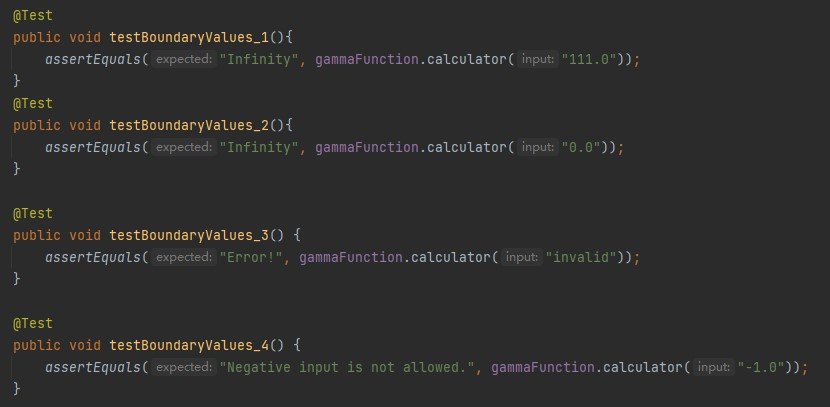
\includegraphics[width=5.5cm]{test_2}
    }
    \subfigure[test3]{
	 		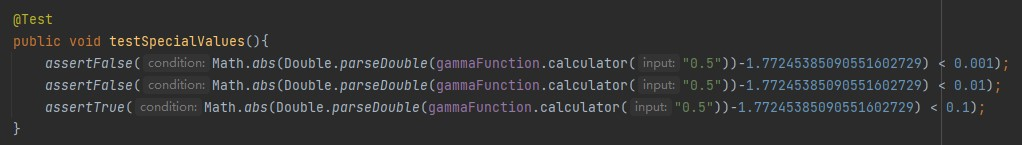
\includegraphics[width=5.5cm]{test_3}
    }
    \caption{Test for boundary and special values}
\end{figure}
\newpage
Finally, I also tested all the sub-functions associated with the gamma function in Algorithm 2, and all the functions were calculated with an error of less than 0.001, as required. As shown in Figure 7:
\begin{figure}[htbp]
\centering
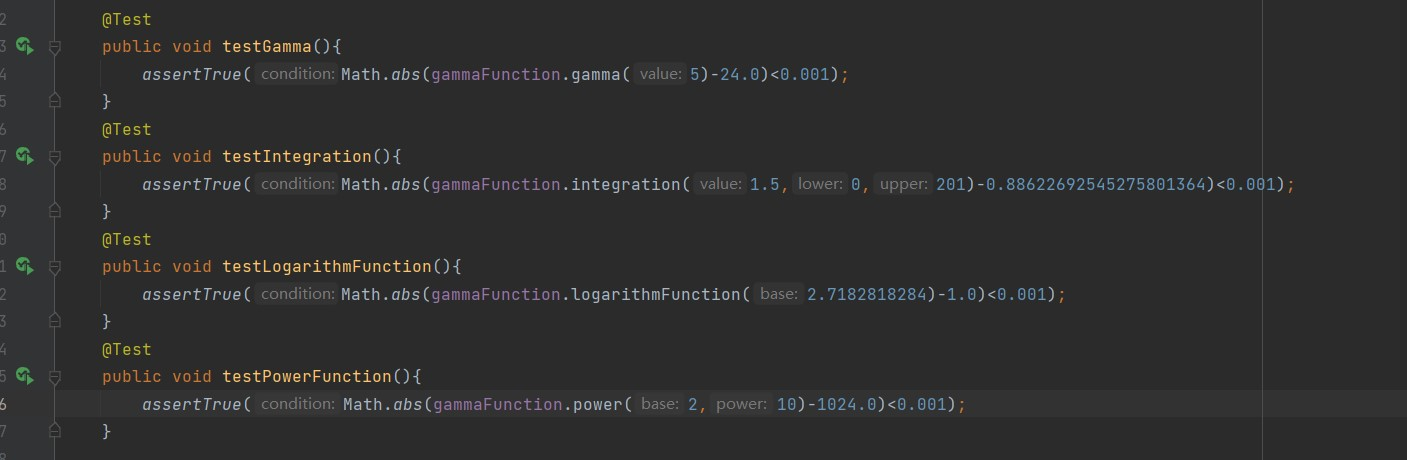
\includegraphics[width=0.75\textwidth]{test_4}
\caption{sub-functions test}
\end{figure}




\bibliographystyle{unsrt}
\bibliography{reference}

\end{document}

